\chapter{Intelligent Agents and MAS}

Nowadays, more and more devices are present in every imaginable context, along with an increasing number of interconnections between them. Moreover, smarter tasks and a tendency to make computers behave like humans are also being pursued.

A software, to support these trends, needs to:
\begin{itemize}
    \item be independent;
    \item Seek the required goals autonomously;
    \item interact with other systems and humans.
\end{itemize}

To build agents capable of such tasks, they need to be endowed with some level of \textbf{intelligence} and \textbf{interaction}, not only independent, autonomous and able to solve the delegated task.

\begin{definitionblock}[Intelligent Agent]
    An agent is a computer system capable of acting \textbf{autonomously} and \textbf{flexibly} in an environment to achieve the assigned objectives.
\end{definitionblock}

\begin{figure}[H]
    \centering
    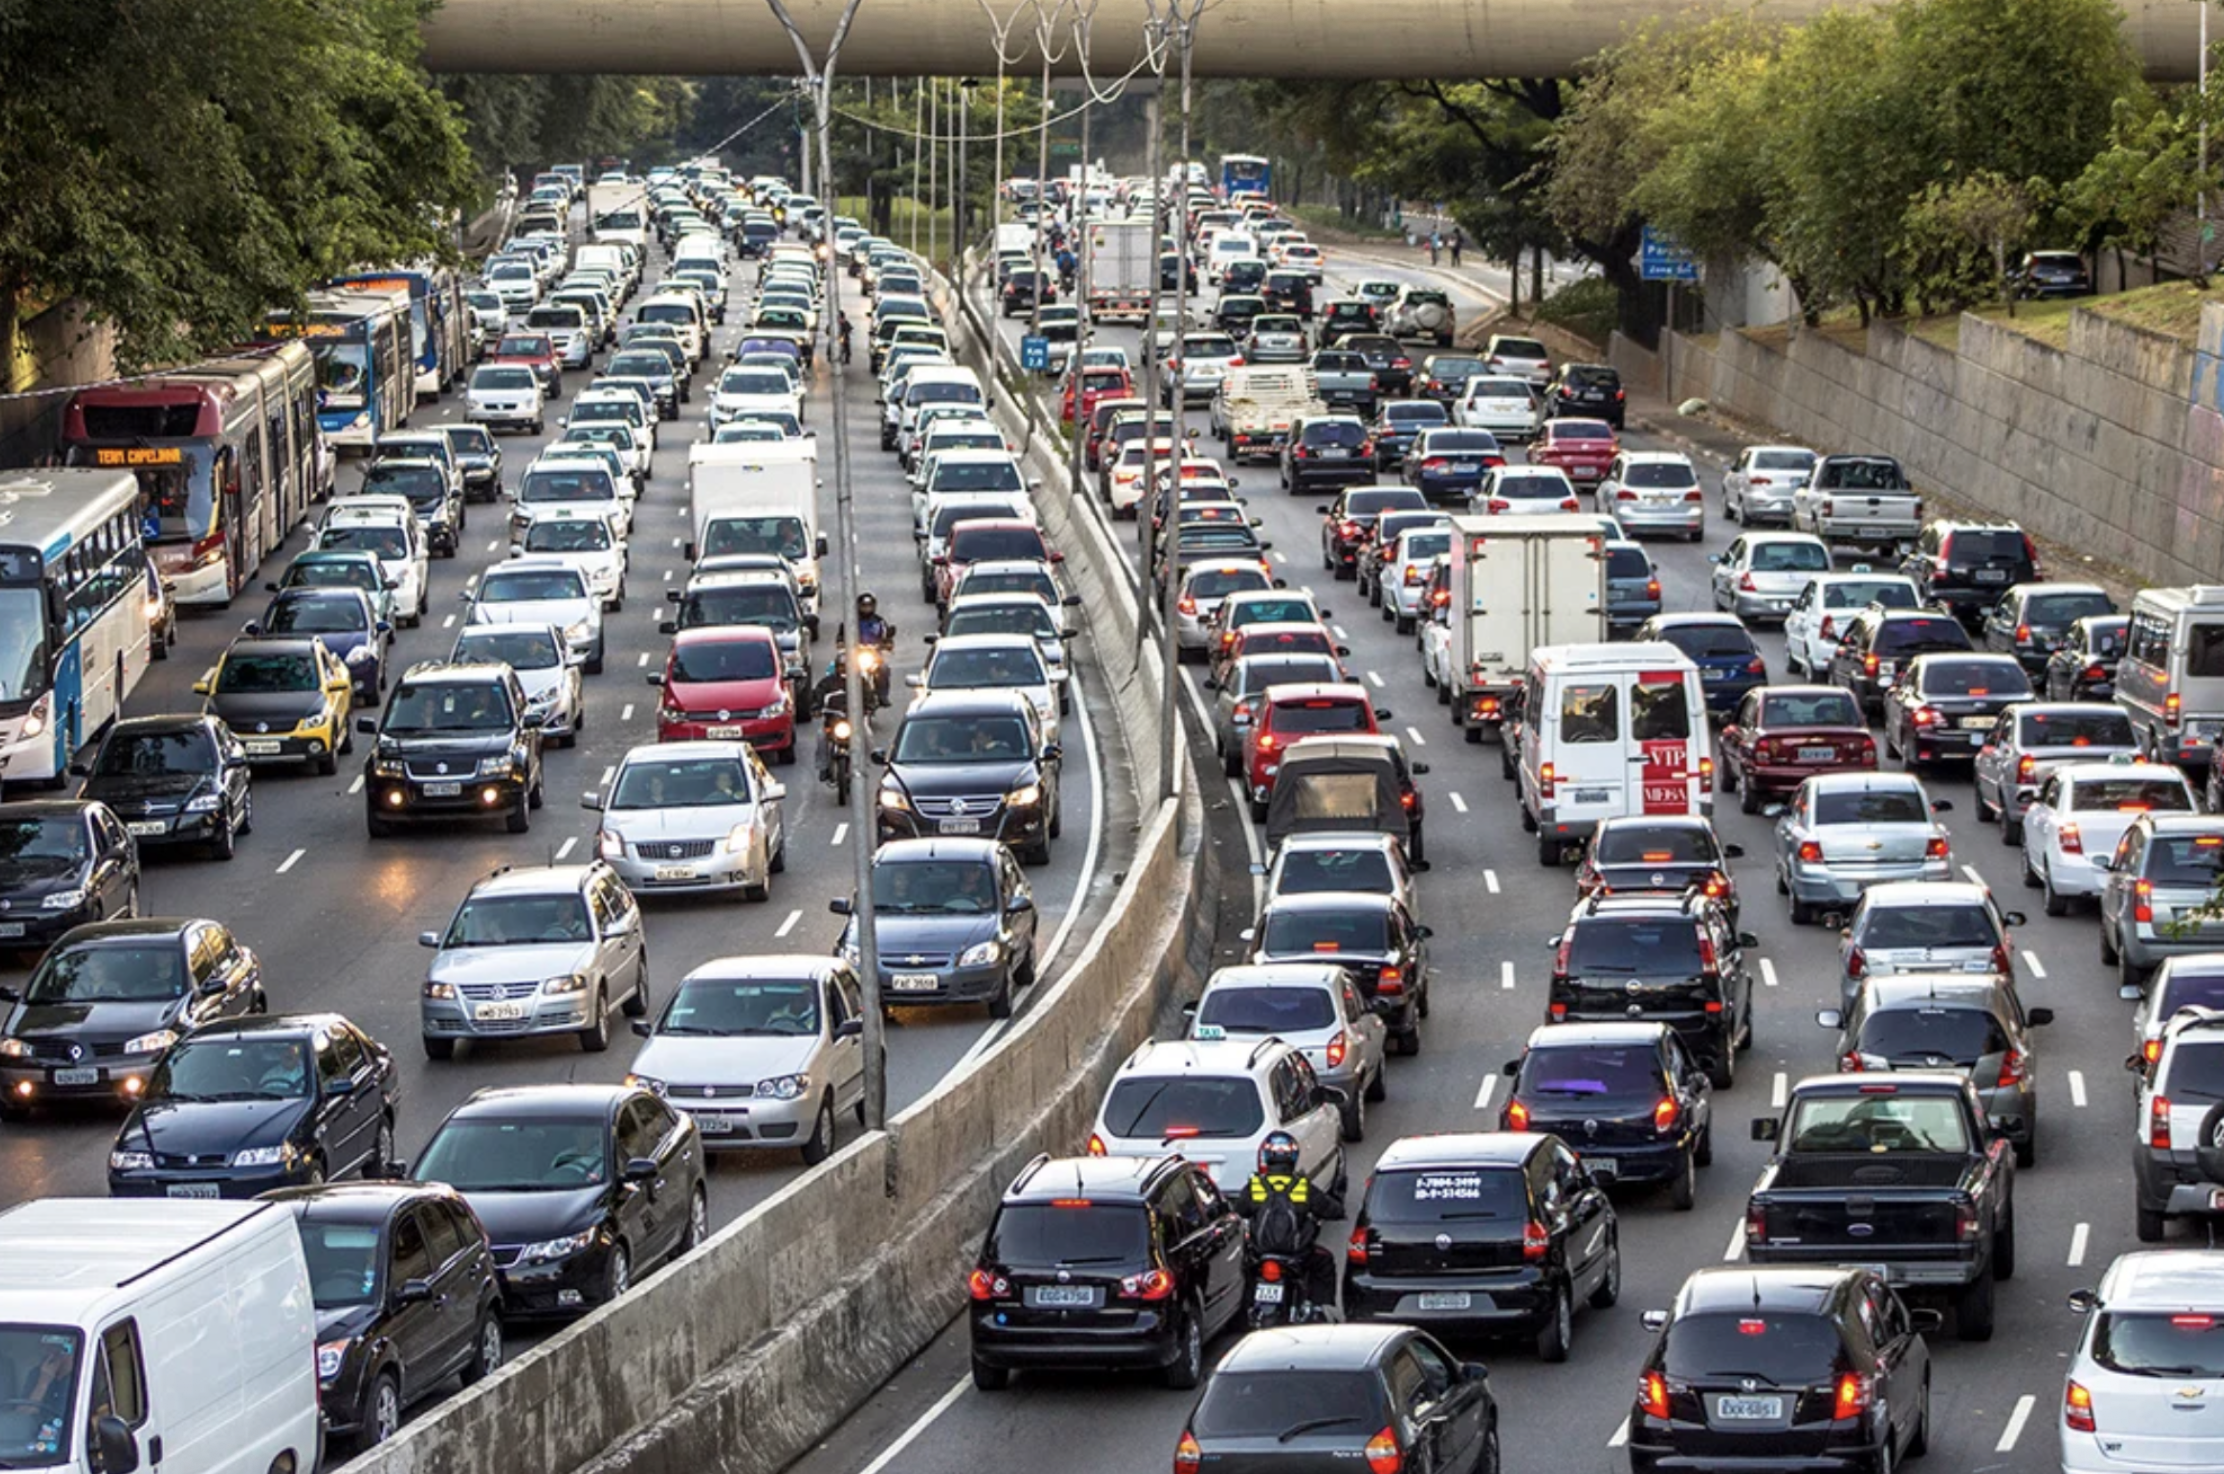
\includegraphics[width=0.8\textwidth]{assets/ch2/1.png}
    \caption{Intelligent Agent}
    \label{fig:intelligent_agent}
\end{figure}

An agent is made by:
\begin{itemize}
    \item \textbf{Perception $P$}: agent's inputs. Perception adjusts the agent's state $S$;
    \item \textbf{State $S$}: internal representation of the world;
    \item \textbf{Action $A$}: agent's output, acting in the environment.
\end{itemize}

Moreover, an agent must be \textbf{flexible}, meaning reactive, proactive and social.
Environmments, instead, must be:
\begin{itemize}
    \item \textbf{Observable}: the agent can acquire complete information;
    \item \textbf{Deterministic}: given an action, we know the resulting state;
    \item \textbf{Episodic}: an action depends on a limited number of previous states;
    \item \textbf{Static}: the environment does not change while the agent is acting;
    \item \textbf{Discrete}: the environment can be divided into distinct states.
\end{itemize}

\begin{figure}[H]
    \centering
    \includegraphics[width=0.8\textwidth]{assets/ch2/2.png}
    \caption{Agent Environment Types}
    \label{fig:agent_environment_types}
\end{figure}

It can be mathematically formalized as a tuple of four components:
\begin{equation*}
    \text{Agent} = \langle P, A, S, f \rangle
\end{equation*}
where:
\begin{itemize}
    \item $P$ is the set of perceptions;
    \item $A$ is the set of actions;
    \item $S$ is the set of internal states;
    \item $f: (P \times S \times A)$ is the state transition function.
\end{itemize}

$S$ is updated base on the actions $A$ taken and the observations $P$ made. $P$ is used to update the agent's internal state $S$ (internal model of the world). $A$ is generated from the agent's state $S$ and current perception $P$. The function responsible for this mapping is called the \textbf{agent function} and referred as $\pi$ (often a probability distribution).

The agent can have a performance evaluation function that measures how well it is performing in achieving its goals. This function can be used to guide the agent's decision-making process and improve its performance over time. Usually a \textbf{reward function $R$} is used to provide feedback to the agent about the desirability of its actions.

The agent's objective is to maximize the cumulative reward over time, which can be formalized as:
\begin{equation*}
    \max_{\pi} \sum_{t=0}^{\infty} \gamma^t R(s_t, a_t)
\end{equation*}
where:
\begin{itemize}
    \item $s_t$ is the state at time $t$;
    \item $a_t$ is the action taken at time $t$;
    \item $\gamma$ is a discount factor (between 0 and 1) that determines the importance of future rewards.
\end{itemize}   

To achieve this, the state-value function $V(s)$ is used to estimate the expected cumulative reward starting from state $s$ and following a particular policy $\pi$:
\begin{equation*}
    V^{\pi}(s) = \mathbb{E}_{\pi} \left[ \sum_{t=0}^{\infty} \gamma^t R(s_t, a_t) \mid s_0 = s \right]
\end{equation*}
where $\mathbb{E}_{\pi}$ denotes the expected value given that the agent follows policy $\pi$.

The policy $\pi(a|s)$ is a function that assigns a state $s$ and a perception $p$ to an action $a$ of the agent, i.e., $\pi: S \times P \rightarrow A$. The agent's objective is to find the optimal policy $\pi^*$ that maximizes the state-value function:
\begin{equation*}
    \pi^* = \arg\max_{\pi} V^{\pi}(s)
\end{equation*}
for all states $s$.

The agent's interaction with the environment can be described in terms of a perception-action cycle. In each cycle, the agent receives a perception from the environment, updates its internal state based on the perception and the action taken, and selects a new action to perform in the environment. 

The selection of the action can be made through a policy function that maps the agent's internal state to a probability distribution over the possible actions. The policy function can be either deterministic or stochastic, depending on whether the agent always selects the same action for a given state or selects actions based on a probability distribution.

\paragraph{Simple Reactive Agents} A reactive agent has a state transition function thet depends solely on the current perception, i.e., $\pi: P \rightarrow S$. It may have (simple) states that will be used to generate actions. If it has no states, then it is called a \textbf{simple reflex agent} and $\pi: P \rightarrow A$. The agent's policy depends only on the current state of the world, ignoring the history of perceptions.

These agents select actions based on the current perceptions, ignoring the rest of the perceptual history. The agent uses a set of condition-action rules, often known as production rules, to determine its action.

\begin{exampleblock}[Simple Reflex Agent]
    Consider a thermostat agent:
    \begin{itemize}
        \item $S$ is boolean and indicates whether the room temperature is too high or too low;
        \item $P$ is the room temperature;
        \item $A$ is either "turn heater on" or "turn heater off";
        \item $f$ compares the current room temperature $P$ with the desired temperature stored in $S$ to decide the appropriate action $A$.
        \item $\pi$ decides the action based on the current perception and the internal state.
    \end{itemize}
\end{exampleblock}

\paragraph{Model-based Reactive Agents} They use a more complex model ($S$) than the previous ones. They take into account the decision of the action to take, maybe using historical data stored in $S$. $A$ is generated from the state $S$ and the agent's current perception $P$ using the policy function $\pi: P \times S \rightarrow A \times S$.
These agents maintain some type of internal model of the world, which allows them to take into account areas that they cannot currently perceive. The model also enables agents to anticipate the outcome of actions in situations where perceptions are insufficient.

\begin{exampleblock}[Model-based Reflex Agent]
    Consider a chess-playing agent:
    \begin{itemize}
        \item $P$ is the move text and turn;
        \item $A$ is the valid piece moves;
        \item $S$ is the internal representation of the chessboard and pieces;
        \item $f$ is the chess rules to determine if an action is legal and to update the board state after $a$;
        \item $\pi$ is the game model and the strategy to select the best move based on the current board state and perception.
    \end{itemize}
\end{exampleblock}

\paragraph{Deliberative Agents} They have an internal component that maintains a model of the world. They use that model to make decisions, being more ambitious than reactive agents. Their state transition function is more complex and depends on both the current perception and the agent's internal world model. The tuple can be written as $\langle P,A,S,f,M\rangle$, where $M$ is the world model. They divide in:
\begin{itemize}
    \item \textbf{Goal-based}: agents that act to achieve specific goals, using their internal model to evaluate the desirability of different states. Planning involves finding the best sequence of actions to achieve the agent's goals;
    \item \textbf{Utility-based}: agents that aim to maximize their expected utility, considering both the likelihood of different outcomes and their preferences over those outcomes.
\end{itemize}

It is important to note that these types of agents are not mutually exclusive, and many agents may combine elements from multiple categories to achieve their objectives effectively. Furthermore, each type of agent may be more suitable for specific tasks or environments, depending on the complexity of the problem and the available resources.

\paragraph{Learning Agents} They have the ability to improve their performance and adapt to changes based on their experience. They usually have five main components:
\begin{itemize}
    \item \textbf{Performance component}: Makes decisions, it is responsible for selecting actions based on perceptions;
    \item \textbf{Learning component}: Responsible for making modifications to the agent to improve performance;
    \item \textbf{Critique component}: This component provides feedback to the learning component about how the agent is performing;
    \item \textbf{Problem generator component}: This component suggests actions that will lead the agent to new and potentially informative experiences;
    \item \textbf{World model}: This component allows the agent to predict how its actions will change the world.
\end{itemize}

\begin{figure}[H]
    \centering
    \includegraphics[width=0.6\textwidth]{assets/ch2/3.png}
    \caption{Learning Agent Architecture}
    \label{fig:learning_agent_architecture}
\end{figure}

\begin{observationblock}[Agents vs Objects]
    Agents differ from traditional objects in several key ways:
    \begin{itemize}
        \item \textbf{Autonomy}: Agents operate independently and make decisions without direct human intervention, while objects typically require external control.
        \item \textbf{Proactivity}: Agents can take initiative to achieve their goals, whereas objects are generally passive and respond only to external stimuli.
        \item \textbf{Social Ability}: Agents can interact and communicate with other agents or humans, while objects usually lack this capability.
        \item \textbf{Adaptability}: Agents can learn from their experiences and adapt their behavior over time, while objects typically have fixed behaviors defined by their programming.
    \end{itemize}
\end{observationblock}

\begin{definitionblock}[BDI Agents]
    BDI agents are a class of deliberative agents that take into account both the agent's knowledge of the world and its goals and plans to make decisions.
\end{definitionblock}

The main components of a BDI agent are:
\begin{itemize}
    \item \textbf{Beliefs (what it knows)}: Information the agent has about the world, itself, and other agents. This knowledge can be incomplete or incorrect.
    \item \textbf{Desires (what it wants)}: The objectives or goals the agent aims to achieve. Desires represent the agent's motivations and can sometimes conflict with each other.
    \item \textbf{Intentions (what it plans to do)}: The plans and actions the agent has committed to in order to achieve its desires. Intentions guide the agent's behavior and decision-making process.
\end{itemize}

There are also behavioral structures that define how BDI agents operate:
\begin{itemize}
    \item \textbf{Perception}: The agent perceives changes in the environment and updates its beliefs accordingly;
    \item \textbf{Rule}: A function that runs in each iteration to infer new desires or beliefs from the agent's current beliefs and desires;
    \item \textbf{Plan}: Defined intensions that the agent can execute to achieve its desires.
\end{itemize}

The BDI agent begins with a set of beliefs and desires. It then uses a reasoning process to generate intentions and select an action to perform based on its current beliefs and intentions. After executing the action, the agent updates its beliefs based on the new information received from the environment, and the cycle continues.

\section{Communication}

In communication, common terms are needed to describe domains and tasks. For example, what do we mean by 'size' or 'fast'? \textbf{Ontologies} offer a shared basis of understanding for agents to communicate effectively.

\begin{definitionblock}[Ontology]
    An ontology is a formal representation of a set of concepts within a domain and the relationships between those concepts. It provides a shared vocabulary and structure for agents to communicate and reason about the domain.
    Ontologies are used in various fields, including artificial intelligence, knowledge representation, and information science, to facilitate interoperability and data sharing among different systems.
\end{definitionblock}

They allow for the estabilisment of common terminology and define relationships between concepts, helping to ensure that agents have a shared understanding of the message they exchange. 

Ontologies typically contain a structural component that is the \textit{taxonomy} of classes and subclass relationships, along with the definitions of the relationships between them. 

\begin{observationblock}[Isn't it a database?]
    Well... not exactly. An ontology captures the semantics and relationships within the domain, while the field desciption in the database focuses on the structure and basic data types needed to store the data. They have significant differences in terms of structure and purpose:
    \begin{itemize}
        \item \textbf{Purpose}: Ontologies are designed to represent knowledge and facilitate reasoning about a domain, while databases are primarily used for storing and retrieving data efficiently.
        \item \textbf{Structure}: Ontologies use classes, properties, and relationships to model complex relationships and hierarchies, while databases use tables, rows, and columns to organize data.
        \item \textbf{Semantics}: Ontologies capture the meaning and context of the data, enabling reasoning and inference, while databases focus on the syntactic representation of data without inherent semantics.
    \end{itemize}
\end{observationblock}

An ontology consists of several components that work together to capture the knowledge and structure of a specific domain. The main components are:
\begin{itemize}
    \item Classes and Class Hierarchies;
    \item Instances;
    \item Properties;
    \item Constraints;
    \item Rules;
    \item Axioms.
\end{itemize}

Where the first two represent the different types of objects in a domain. An instance is an object of the class.

\paragraph{Properties} They define attributes or relationships between classes in an ontology. Properties can have a \textit{domain} (the class to which the property applies) and a \textit{range} (the type of value that the property can have). There are two main types of properties:
\begin{itemize}
    \item \textbf{Instances}: describe characteristics of individual instances of classes;
    \item \textbf{Relations}: describe relationships between different classes or instances.
\end{itemize}

\begin{exampleblock}[Properties]
    \begin{codeblock}
Instance property: name (domain: Animal, range: string)
Relation property: hasParent (domain: Person, range: Person)
    \end{codeblock}
\end{exampleblock}

\paragraph{Restrictions} Impose conditions or rules on the classes and properties in an oncology. These restrictions can include cardinality constraints, range restrictions, allowed value restrictions, among others. 
\begin{exampleblock}[Restrictions]
    \begin{codeblock}
Cardinality restriction: A Person must have exactly two parents.
Range restriction: The age property of a Person must be an integer between 0 and 120.
    \end{codeblock}
\end{exampleblock}

\paragraph{Rules} Rules allow for the definition of additional logic or inferences within an ontology. They can be logical rules or rules based on the semantics of concepts and relationships within the domain. 
\begin{exampleblock}[Rules]
    \begin{codeblock}
If a Person is a Parent, then they must have at least one Child.
If an Animal is a Mammal, then it must give birth to live young.
    \end{codeblock}
\end{exampleblock}

\paragraph{Axioms} Axioms are statements that establish fundamental truths or assumptions within an ontology. They provide additional information and constraints about classes, properties and relationships in the domain. Axioms can be of different types: \textit{equivalence}, \textit{inheritance} and \textit{restriction}.

\begin{exampleblock}[Axioms]
    \begin{codeblock}
Equivalence axiom: A Bachelor is equivalent to an Unmarried Man.
Inheritance axiom: All Dogs are Animals.
Restriction axiom: A Person can have at most two biological parents.
    \end{codeblock}
\end{exampleblock}

\subsection{Communication Acts}

How do we exchange messages between agents? Communication acts are a way to structure the messages that agents exchange, i.e., 'request', 'report', 'confirmation', 'negotiation', etc. Ontologies can include communication acts. These definitions allow agents to understand the purpose and intention behind messages and to engage in negotiations and coordination of actions. By using the ontology to interpret communication acts, agents can make decisions based on the underlying semantics and coordinate their actions more effectively. They are typically defined using a communication protocol that specifies the syntax and semantics of the messages exchanged between agents.

Communication languages are a set of rules that agents use to communicate with each other. They define the syntax and semantics of the messages exchanged between agents, allowing them to understand each other's intentions and actions. Examples of communication languages include KQML (Knowledge Query and Manipulation Language) and FIPA ACL (Foundation for Intelligent Physical Agents Agent Communication Language). Communication languages specify how messages are structured and what the different communication acts mean. 

\begin{itemize}
    \item \textbf{Ontology} provides a common semantic structure and definitions of concepts;
    \item \textbf{Communication language} establishes the rules and format for message exchange. 
\end{itemize}

Together, they enable semantic interoperability, precise communication and shared understanding between agents. 

\paragraph{KQML} Developed in the 1990s, it is still used toda in some systems. It defines a syntax for messages and a set of predefined communication acts. Here, structured messages are used to query and manipulate knowledge between agents.

\begin{exampleblock}[KQML Message]
    \begin{codeblock}
(Send
    :receiver AgentB
    :content (ask-one
                :receiver all
                :content (predicate "p" :arg1 "x")))

(Tell
    :sender AgentB
    :content (result 
                :in-reply-to (ask-one :receiver all :content (predicate "p" :arg1 "x")
                :content "Yes")))
    \end{codeblock}
\end{exampleblock}

In practice, various types of messages and actions can be used to perform more complex queries and manipulate knowledge between agents. KQML is a specific communication language: the agents involved must understand and process the messages in KQML format.

\paragraph{FIPA ACL} ACL is another communication language that includes a broader set of communication acts and more sophisticated protocol mechanisms than KQML. 
\begin{exampleblock}[FIPA ACL Message]
    \begin{codeblock}
(REQUEST
    :sender (agent-identifier :name AgentA :addresses (sequence AgentA-address))
    :receiver (set (agent-identifier :name AgentB :addresses (sequence AgentB-address)))
    :content "System status?")
(INFORM
    :sender (agent-identifier :name AgentB :addresses (sequence AgentB-address))
    :receiver (set (agent-identifier :name AgentA :addresses (sequence AgentA-address)))
    :content "All systems operational.")
    \end{codeblock}
\end{exampleblock}

FIPA is an international organization dedicated to promoting and standardizing technologies related to Intelligent Agents. It focuses on developing standards and specifications to facilitate interoperability and information exchange among intelligent agents. 
\begin{itemize}
    \item \textbf{Standards and specifications}: FIPA develops technical standards and specifications that establish a common framework;
    \item \textbf{Interoperability}: FIPA standards enable intelligent agents from different platforms and systems to communicate and collaborate effectively;
    \item It was a key organization in promoting and standardizing technologies related to intelligent agents.
\end{itemize}

Examples of FIPA protocols include:
\begin{table}[H]
\centering
\begin{tabular}{|c|p{8cm}|}
\hline
\textbf{Protocol} & \textbf{Description} \\
\hline
FIPA Request & An agent requests another agent to perform a specific action or task. \\
\hline
FIPA Contract Net & A negotiation protocol where an agent announces a task and other agents bid to perform it. \\
\hline
FIPA Subscribe & An agent subscribes to receive updates or notifications from another agent about specific events or changes. \\
\hline
FIPA Query & An agent queries another agent for information or data. \\
\hline
\end{tabular}
\caption{FIPA Protocols}
\label{tab:fipa_protocols}
\end{table}

\begin{exampleblock}[Request-proposal protocol]
    An agent requests a task from another agent and receives a proposal on how the task will be carried out. The requesting agent sends a \plaintt{request} message that includes the details of the task being requested. The agent receiving the request sends a \plaintt{proposal} message that includes an offer to perform the task and the details of how it will be carried out. 
\end{exampleblock}

Within a FIPA communication protocol, agents can perform different communication acts. These acts include requesting information, making proposals, accepting or rejecting offers, notifying events and more. Agents carry out these acts using the messages and rules defined in the protocol. 

\section{Interacting through cooperation}

\subsection{Cooperation}

Cooperation among intelligent agents is essential for achieveing shared goals. Agents need to share \textbf{information}, \textbf{assign tasks}, \textbf{make joint decisions} and \textbf{coordinate actions}. Cooperation can be challenging due to differences in the capabilities and knowledge of the agents, as well as the possibility of \textbf{selfish} or \textbf{malicious behavior}. 

\begin{observationblock}[Difference from traditional distributed systems]
    In traditional distributed systems, components work together to achieve a common goal, often relying on centralized control and predefined protocols. In contrast, multi-agent systems consist of autonomous agents that interact and cooperate in a decentralized manner, often with varying degrees of knowledge and capabilities.
\end{observationblock}

\textbf{Cooperative Distributed Problem Solving (CDPS)} studies how a network of solvers can work together to solve problems that are beyond their individual capabilities. Each node in the network is capable of solving problems in a sophisticated and independent manner, but cannot complete them without cooperation. \textbf{Benevolence} is assumed, meaning that the nodes implicitly share a common goal (no conflict among them). 

\begin{itemize}
    \item \textbf{Coherence} refers to how well the multi-agent system behaves as a unit across some dimension of evaluation;
    \item \textbf{Coordination} refers to the degree to which agents can avoid individual activities by synchronizing and aligning their actions. 
\end{itemize}

In a perfectly coordinated system, agents will not accidentally interfere with each other's sub-goals while attempting to achieve a common goal. 

\paragraph{Task Sharing} The problem is decomposed into subproblems and assigned to different agents. Task assignment to individual agents may involve agreements, neegotiations or auctions. 

\textbf{Task assignment} is a key component of cooperation. Tasks must be divided and assigned efficiently to make the most of each agent's capabilities. A common approach is the \textbf{Contract Net Protocol (CNP)}, which is an auction protocol in which agents are either \textbf{manager} or \textbf{contractor}.

\begin{enumerate}
    \item \textbf{Task Announcement}: The manager agent announces a task to be performed, specifying the requirements and constraints;
    \item \textbf{Bids}: Contractor agents evaluate the task and submit bids, indicating their willingness to perform the task and the associated cost or resources required;
    \item \textbf{Task Assignment}: The manager agent evaluates the bids and selects the most suitable contractor based on criteria such as cost, quality or timeliness. The task is then assigned to the selected contractor;
    \item \textbf{Task Execution}: The contractor agent performs the assigned task and reports the results back to the manager agent upon completion.
\end{enumerate}
\begin{center}
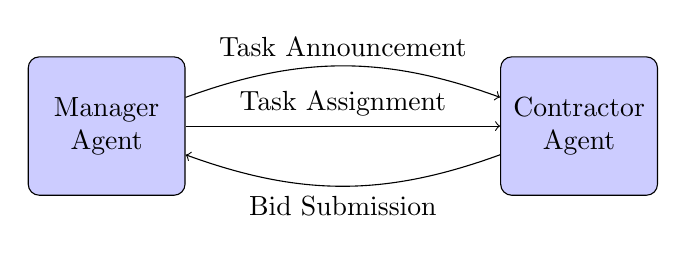
\begin{tikzpicture}[
    node distance=3cm, 
    auto,
    block/.style={rectangle, draw, fill=blue!20, text width=5em, text centered, rounded corners, minimum height=5em}
]
    \node[block] (manager) {Manager Agent};
    \node[block, right of=manager, node distance=6cm] (contractor) {Contractor Agent};
    
    \draw[->, bend left=20] (manager) to node[above] {Task Announcement} (contractor);
    \draw[->] (manager) -- node[above] {Task Assignment} (contractor);
    \draw[->, bend left=20] (contractor) to node[below] {Bid Submission} (manager);
\end{tikzpicture}
\end{center}

The CNP is a decentralized mechanism, meaning there is no single point of control of failure. It is flexible and can adapt to a wide variety of situations and needs. However, the effectiveness of the CNP can be affected by the quality of the bids and the agents' ability to evaluate and select the best offers. The best strategy for bidding and task assignment may vary depending on the specific context and requirements of the system.

\paragraph{Result Sharing} Agents share subproblem information proactively and reactively. This is useful when agents have different knowledge or capabilities.
 
Sharing results is a method in which agents cooperatively exchange information while developing a solution. These initial results are often the solution to small problems, which are then refined into larger and more abstract solutions. Problem solvers can improve the group's performance in sharing results:
\begin{itemize}
    \item \textbf{Trust}: Independently derived solutinos can be verified against each other, highlighting potential errors and increasing confidence in the overall solution;
    \item \textbf{Completeness}: Sharing their local views to achieve a better global perspective;
    \item \textbf{Accuracy}: Sharing results to ensure that the accuracy of the global solution is increased;
    \item \textbf{Timeliness}: Although an agent could solve a problem by itself, by sharing a solution, the result could be derived more quickly.
\end{itemize}

\begin{warningblock}[Inconsistencies]
    Agents may have inconsistencies regarding their beliefs and their goals/intentions. Inconsistencies between goals generally arise because agents are assumed to be autonomous and therefore do not share common objectives and they are a major problem in cooperative systems.
    There are several sources of inconsistencies:
    \begin{itemize}
        \item The perspective that agents have will typically be limited;
        \item The sensors that agents have may be faulty, or the sources of information to which the agent has access may be faulty.
    \end{itemize}
\end{warningblock}

\subsection{Coordination}

It refers to the management of the interdependencies between the activities of agents. They may have a positive relationship (beneficial for at least one agent) or a negative relationship (destructive for at least one agent). Coordination in MAS is assumed to occur in real-time and agents must be able to recognize and manage these relationships during their activities. There are different types of coordination among agents:

\paragraph{Partial Global Planning} Involves agents generating and following a global plan that only covers part of their activities. It is used when it is not feasible or efficient to plan all activities of all agents due to complexity of the system. 

\begin{exampleblock}
    In public transportation, buses and trains may have their own schedules and routes, but they also need to coordinate with each other to ensure smooth transfers for passengers. Partial global planning allows each mode of transportation to plan its own activities while still considering the overall system's needs.
\end{exampleblock}

\begin{itemize}
    \item \textbf{Pros}: Allows for high efficiency in task resolution and high coherence in decision making;
    \item \textbf{Cons}: Requires good communication and synchronization among agents and is not ideal for highly dynamic or uncertain environments where plans may need to be changed frequently.
\end{itemize}

\paragraph{Joint Intentions} Agents form and act upon intentions that are shared among them. They commit to working together toward a common goal and to communicate with each other about their intentions and actions. 

\begin{exampleblock}
    In a search and rescue operation, multiple agents (e.g., drones, robots, and human responders) may form joint intentions to locate and assist survivors. They share information about their findings and coordinate their actions to cover the search area effectively.
\end{exampleblock}

\begin{itemize}
    \item \textbf{Pros}: Enhances cooperation and coordination among agents, leading to more effective problem-solving;
    \item \textbf{Cons}: Requires a high level of trust and communication among agents, which may not always be feasible in dynamic or uncertain environments, especially with a large number of agents or with conflicting goals.
\end{itemize}

\paragraph{Mutual Modeling} Involves agents building and using models of each other to anticipate their actions and coordinate their own actions accordingly. 

\begin{exampleblock}
    In a team of autonomous vehicles, each vehicle may use mutual modeling to predict the movements and intentions of other vehicles on the road. This allows them to coordinate their actions, such as merging or changing lanes, to ensure safe and efficient traffic flow.
\end{exampleblock}

\begin{itemize}
    \item \textbf{Pros}: Enables agents to anticipate and adapt to each other's actions, leading to more effective coordination in dynamic and complex environments;
    \item \textbf{Cons}: Requires accurate and up-to-date models of other agents, which could be expensive in computational terme and lead to errors if the models are not accurate.
\end{itemize}

\paragraph{Social Norms and Laws} Agents follow established social norms and laws to guide their behavior and interactions with each other.
\begin{exampleblock}
    In a multi-agent system for online marketplaces, agents representing buyers and sellers may adhere to social norms and laws regarding fair pricing, honest communication, and dispute resolution. This helps maintain trust and cooperation among participants.
\end{exampleblock}

\begin{itemize}
    \item \textbf{Pros}: Provides a clear framework for agent behavior, promoting cooperation and reducing conflicts;
    \item \textbf{Cons}: May limit agent autonomy and flexibility, especially in dynamic or uncertain environments where norms and laws may need to be adapted.
\end{itemize}

\subsection{Planning}

Planning in multi-agent systems involves the coordination and collaboration of multiple agents to achieve shared goals. Each agent may have its own individual goals and plans, but they must also consider the actions and plans of other agents in the system. There are three main approaches to planning in multi-agent systems:

\paragraph{Centralized Planning for Distributed Plans} Develops a plan for a group of agents, where the division and order of work are defined. This plan is distributed among the agents, who execute their part of the plan. 

\begin{itemize}
    \item \textbf{Pros}: Allows for coordination and efficiency, having a single centralized agent with a global view efficiently assigning tasks to agents;
    \item \textbf{Cons}: If the centralized planner fails, the entire system may be compromised; it may not scale well with a large number of agents or in geographically dispersed systems or those with private information that cannot be shared with a central planner.
\end{itemize}

\paragraph{Distributed Planning} A group of agents cooperate to form a centralized plan. The agents forming the plan will not be the ones executing it. 

\begin{itemize}
    \item \textbf{Pros}: Planning is more robust to failures and is more suitable if agents have private or dispersed information;
    \item \textbf{Cons}: The challenge is to coordinate the actions of agents to avoid conflicts. Moreover, it is more difficult to achieve an efficient plan (lack of global view).
\end{itemize}

\paragraph{Distributed Planning for Distributed Plans} A group of agents cooperates to form individual action plans, dynamically coordinating their activities. When coordination problems arise, they may need to be resolved through negotiation.

\begin{itemize}
    \item \textbf{Pros}: More flexible and scalable, as agents can create and execute their own plans independently, is also more suitable for situations where agents have private information;
    \item \textbf{Cons}: Need for sophisticated mechanisms for coordination and conflict resolution among agents' plans.
\end{itemize}

\subsection{Coalitions}

\begin{definitionblock}[Coalition]
    A coalition is a subset of agents that work together to achieve common goals. They allow for the distribution of tasks and collaboration to improve efficienct and achieve goals that cannot be reached individually.
\end{definitionblock}

Coalitions are situated in both coordination and planning of MAS:
\begin{itemize}
    \item \textbf{Coordination}: Coalition agents must coordinate to work effectively together;
    \item \textbf{Planning}: Coalition agents must engage in joint planning to achieve their objectives.
\end{itemize}

Agents identify potential allies based on their capabilities and objectives. The terms of cooperation are negotiated, including the division of tasks and rewards. The challenges include determining \textbf{when} and \textbf{how} to form coalitions can be a complex problem and the \textbf{balancing}  of the agents' interests with the benefits of cooperation.

\begin{exampleblock}[Applications of coalitions in MAS]
    \begin{itemize}
        \item \textbf{Resource Management}, where agents cooperate to share resources;
        \item \textbf{Problem-solving}, where agents work toghether to solve complex problems;
        \item \textbf{In dynamics environments}, where agents form and reform coalitions in response to chenges in the environment.
    \end{itemize}
\end{exampleblock}

\subsection{Voting in MAS}

Voting procedures are methods that allow intelligent agents to make collective decisions. Voting is crucial in MAS to facilitate cooperation and collective decision-making. Agents vote to make decisions that affect the entire coalition or the MAS as a whole. 

Voting procedures can vary in \textbf{complexity}, from simple majority voting to weighted voting mechanisms or more complex procedures. Agents can cast their votes based on their \textbf{knowledge}, \textbf{goals} and \textbf{strategies}.

\begin{itemize}
    \item \textbf{Majority Voting}: Each agent casts a vote for a particular option, and the option with the most votes wins;
    \item \textbf{Weighted Voting}: Each agent's vote is assigned a weight based on its importance or expertise, and the option with the highest total weight wins;
    \item \textbf{Consensus Voting}: Agents discuss and negotiate to reach a unanimous decision;
    \item \textbf{Ranked Voting}: Agents rank the options in order of preference, and the option with the highest overall ranking wins.
\end{itemize}

Voting facilitates cooperation and collective decision-making in MAS. It promotes \textbf{fairness} by giving all agents the opportunity to express their preferences and helps resolve conflicts and make decisions in uncertain situations.

\begin{warningblock}[Challenges and considerations]
    Agents may have incentives to manipulate the voting process to achieve their desired outcomes. Designing voting procedures that are robust against strategic manipulation is a significant challenge in MAS and so voting systems must be designed to be resilient to such manipulations. Moreover, the \textbf{computational efficiency} of the voting process must be considered. They should be \textbf{fair} and \textbf{transparent}.
\end{warningblock}

\subsection{Manipulation and Reputation}

Manipulation and reputation are two crucial aspects of MAS. The first can be detrimental to the system's performance, while the second can promote cooperation and discourage selfish or malicious behaviors.

\begin{itemize}
    \item \textbf{Manipulation}: occurs when an agent influences the decision-making of others for personal gain, for example by provising false information to change the outcome of a voting process in their favor; it can have negative consequences for the system as a whole, such as suboptimal decisions or reduced cooperation among agents. It is important to implement mechanisms to prevent manipulations, such as:
    \begin{itemize}
        \item Manipulation-resistant voting procedures;
        \item Secure communication protocols;
        \item Anomaly detection systems.
    \end{itemize}
    \item \textbf{Reputation} is a measure of an agent's past behavior: agents with good reputation are often seen as more reliable and cooperative, while agents with bad reputation may be considered potentially harmful or uncooperative. Reputation can be an effective mechanism to incentivize cooperation and discourage selfish or malicious behaviors. Reputation management involves collecting, storing and sharing information about the past behavior of agents, using a rating system, a trust system or a recommendation system.
\end{itemize}

\begin{warningblock}[Challenges]
    \begin{itemize}
        \item The need to protect the \textbf{privacy} of agents while collecting and sharing reputation information;
        \item The possibility of false or manipulated ratings that can distort the reputation system;
        \item The need to make decisions based on \textbf{incomplete} or \textbf{uncertain} information about agents' behavior.
    \end{itemize}
\end{warningblock}

\section{Competition and Negotiation}

\textbf{Competition} and \textbf{negotiation} are two essential aspects in MAS. Agents may compete for limited resources or negotiate to achieve common goals. 

\paragraph{Competition} It occurs when the agents seek to maximize their individual benefits, often at the expense of others and happen when resources are scarce and agents have opposing interests. 

\paragraph{Negotiation} It is a communication and decision-making process in which agents try to reach an agreement. It can be:
\begin{itemize}
    \item \textbf{Cooperative}, where agents work together to achieve a common goal;
    \item \textbf{Competitive}, where agents have opposing interests and try to maximize their individual benefits.
\end{itemize}

There are several negotiation techniques:
\begin{itemize}
    \item Bilateral negotiation;
    \item Multilateral negotiation;
    \item Auction-based negotiation;
\end{itemize}

The choice of negotiation technique depends on the specific context and requirements of the MAS.

\begin{warningblock}[Challenges in competition and negotiation]
    \begin{itemize}
        \item The need to balance individual interests with the overall goals of the system;
        \item The complexity of negotiation processes, especially in multilateral negotiations;
        \item The possibility of manipulation or deception by agents to gain an advantage.
    \end{itemize}
\end{warningblock}

\textbf{Utility} is a measure of the satisfaction or benefit an agent gains from a process. Agents make decisions based on maximizing their expected utility and an agent's preferences reflect their relative evaluation of different outcomes. \textbf{Preferences} can be represented as a utility function, which assigns a numerical value to each possible outcome. 

Therefore, a \textbf{dominant strategy} is a strategy that provides the agent with the highest utility, regardless of the strategies chosen by other agents. In some games, a dominant strategy may not exist.

\subsection{Game Theory}

\textbf{Dilemmas} and \textbf{Games} are situations where agents interact and make decisions. \textbf{Game Theory} is an essential tool for modeling and analyzing these situations.

\begin{definitionblock}[Game Theory]
    Game theory is the study of mathematical models of strategic interaction among rational decision-makers. It provides a framework for analyzing situations where the outcome of one agent's decision depends on the decisions made by other agents.
\end{definitionblock}

Games can be classified based on several criteria:
\begin{itemize}
    \item \textbf{Number of players}: two-player games, multiplayer games;
    \item \textbf{Information availability}: perfect information games, imperfect information games;
    \item \textbf{Cooperation}: cooperative games, non-cooperative games;
    \item \textbf{Zero-sum vs non-zero-sum}: in zero-sum games, one player's gain is another player's loss, while in non-zero-sum games, both players can benefit from cooperation.
\end{itemize}

And exist different types of games:
\begin{itemize}
    \item \textbf{Cooperative games}: players can form coalitions and share their payoffs;
    \item \textbf{Competitive games}: players compete against each other to maximize their own payoffs;
    \item \textbf{Symmetric games}: players have identical strategies and payoffs;
    \item \textbf{Asymmetric games}: players have different strategies and payoffs.
\end{itemize}

\begin{definitionblock}[Nash Equilibrium]
    A Nash Equilibrium is a solution concept in game theory where no player can improve their outcome by unilaterally changing their strategy, given the strategies of the other players. In other words, it is a stable state in which each player's strategy is optimal, considering the strategies chosen by the other players. 
\end{definitionblock}

Each game can have one, several or no Nash equilibria at all. Finding the Nash equilibria of a game can be a complex task, especially in games with many players and strategies.

\subsection{Auctions}

Auctions are effective mechanisms for \textbf{allocating} scarce resources among multiple agents. They provide a structured way for agents to express their preferences and compete for resources. Intelligent agents can use them to determine the value of a resource and allocate it fairly and efficiently. There are different types of auctions:
\begin{itemize}
    \item \textbf{Common Value}: The value of the item is the same for all bidders (may be uncertain or unknown prior to the auction), but bidders have different information about that value;
    \item \textbf{Private Value}: Each bidder has their own individual valuation of the item, which is independent of other bidders' valuations, and each bidder does not know the valuations of other bidders;
    \item \textbf{Correlated Value}: The value of the item is a blend of private and common value. Bidders have private information that helps them estimate the value of the item. Here, each agent has a private estimate of the value of the item, but these estimates are correlated because they are based on shared common information;
    \item \textbf{Open Cry}: Bidders openly bid against each other, with each bidder able to see the current highest bid and respond accordingly;
    \item \textbf{Sealed Bid}: Bidders submit their bids without knowing the bids of other participants. The highest bid wins, but bidders do not have the opportunity to adjust their bids based on others' offers.
    \item \textbf{One-shot Auction}: Bidders submit their bids only once, and the auction concludes after a single round of bidding;
    \item \textbf{Ascending Auction}: Bidders can place multiple bids, with each bid being higher than the previous one. The auction continues until no higher bids are made.
\end{itemize}

Each auction type has its own advantages and disadvantages, and the choice of auction type depends on the specific context and requirements of the MAS. For example, common value auctions can be useful in situations where the value of a resource is the same for all agents and each agent has an uncertain estimate of that value. 